\documentclass{beamer}
\usetheme{CambridgeUS}
\usecolortheme{spruce}
\usefonttheme{serif}

\usepackage{lipsum}
\usepackage{graphicx,xcolor}
\usepackage{amsmath,amssymb,amsfonts}
\usepackage[utf8]{vietnam}
\usepackage{verbatim,longtable}
\setbeamertemplate{caption}[numbered]

\usepackage{ragged2e}
\usepackage{etoolbox}
% \usepackage{algorithm,algorithmic}
% \usepackage{algorithm2e}
% \usepackage{algpseudocode}
% \usepackage{float}
\usepackage{booktabs}
\usepackage{caption}
\usepackage{blindtext}
\apptocmd{\frame}{}{\justifying}{}
% \addtobeamertemplate{frame begin}{}{\justifying}

\apptocmd{\column}{}{\justifying}{}

\usepackage{subfig}

\AtBeginSection[]{ 
    \begin{frame}{Outline} 
        \tableofcontents[currentsection] 
    \end{frame} }

\title[thesis]{Phương pháp tìm kiếm lân cận rộng thích ứng \\
cho một số lớp bài toán định tuyến phương tiện}
% \subtitle{Luận văn thạc sĩ}
\author[Linh]{Nguyễn Mạnh Linh}
\institute[MIM, HUS]{Khoa Toán-Cơ-Tin học \\ Đại học Khoa học Tự nhiên}
\date{2023/12}
% \titlegraphic{\includegraphics[width=2cm]{images/logo/iiserm_logo.jpg}}

\begin{document}

\begin{frame}
\titlepage
\end{frame}


\section{Giới thiệu}
% \begin{frame}{Giới thiệu}
%     % \begin{figure}
%     % \centering
%     % \includegraphics[scale=0.2]{images/fig_01.png}
%     % \caption{Các mẫu đối nghịch bị phân loại sai
%     %     bởi mô hình Inception-V3}
%     % \end{figure}
% \end{frame}

\begin{frame}{Giới thiệu}
    \begin{figure}[H] % places figure environment here   
        \centering % Centers Graphic
        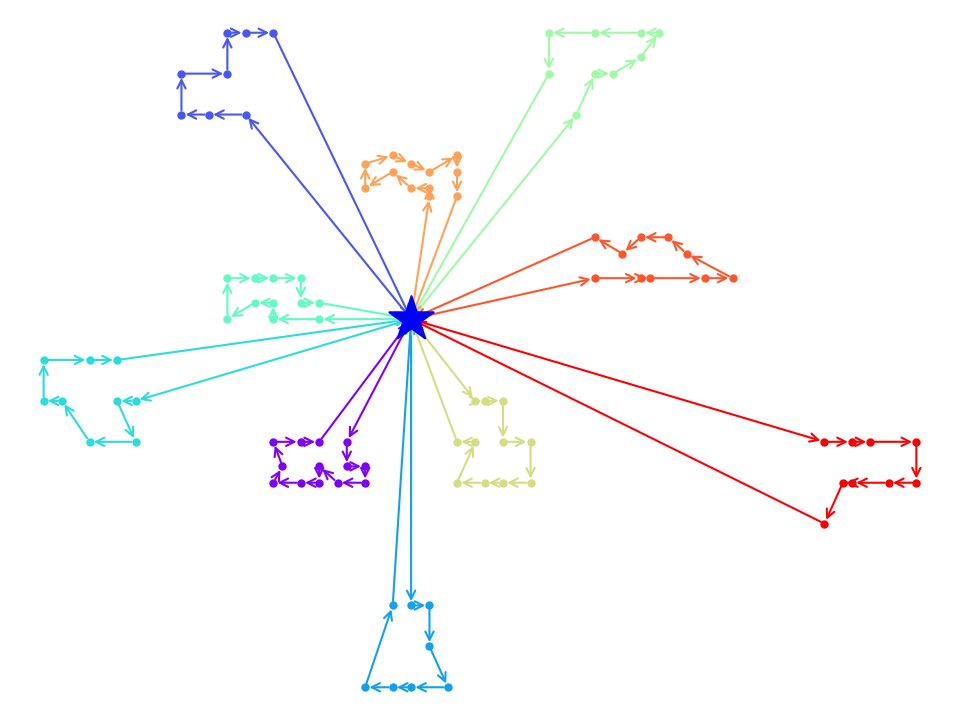
\includegraphics[width=0.6\textwidth]{figures/routes_c101.png} 
        % \includesvg[scale=1]{figures/core-object}
        \caption{VRP với 10 xe phục vụ 100 khách hàng (cấu hình Solomon C101).} 
        % \label{fig:fg_02}
    \end{figure}
\end{frame}

\section{Định nghĩa và một số kí hiệu}
\begin{frame}{Định nghĩa}
    \begin{figure}[H] % places figure environment here   
        \centering % Centers Graphic
        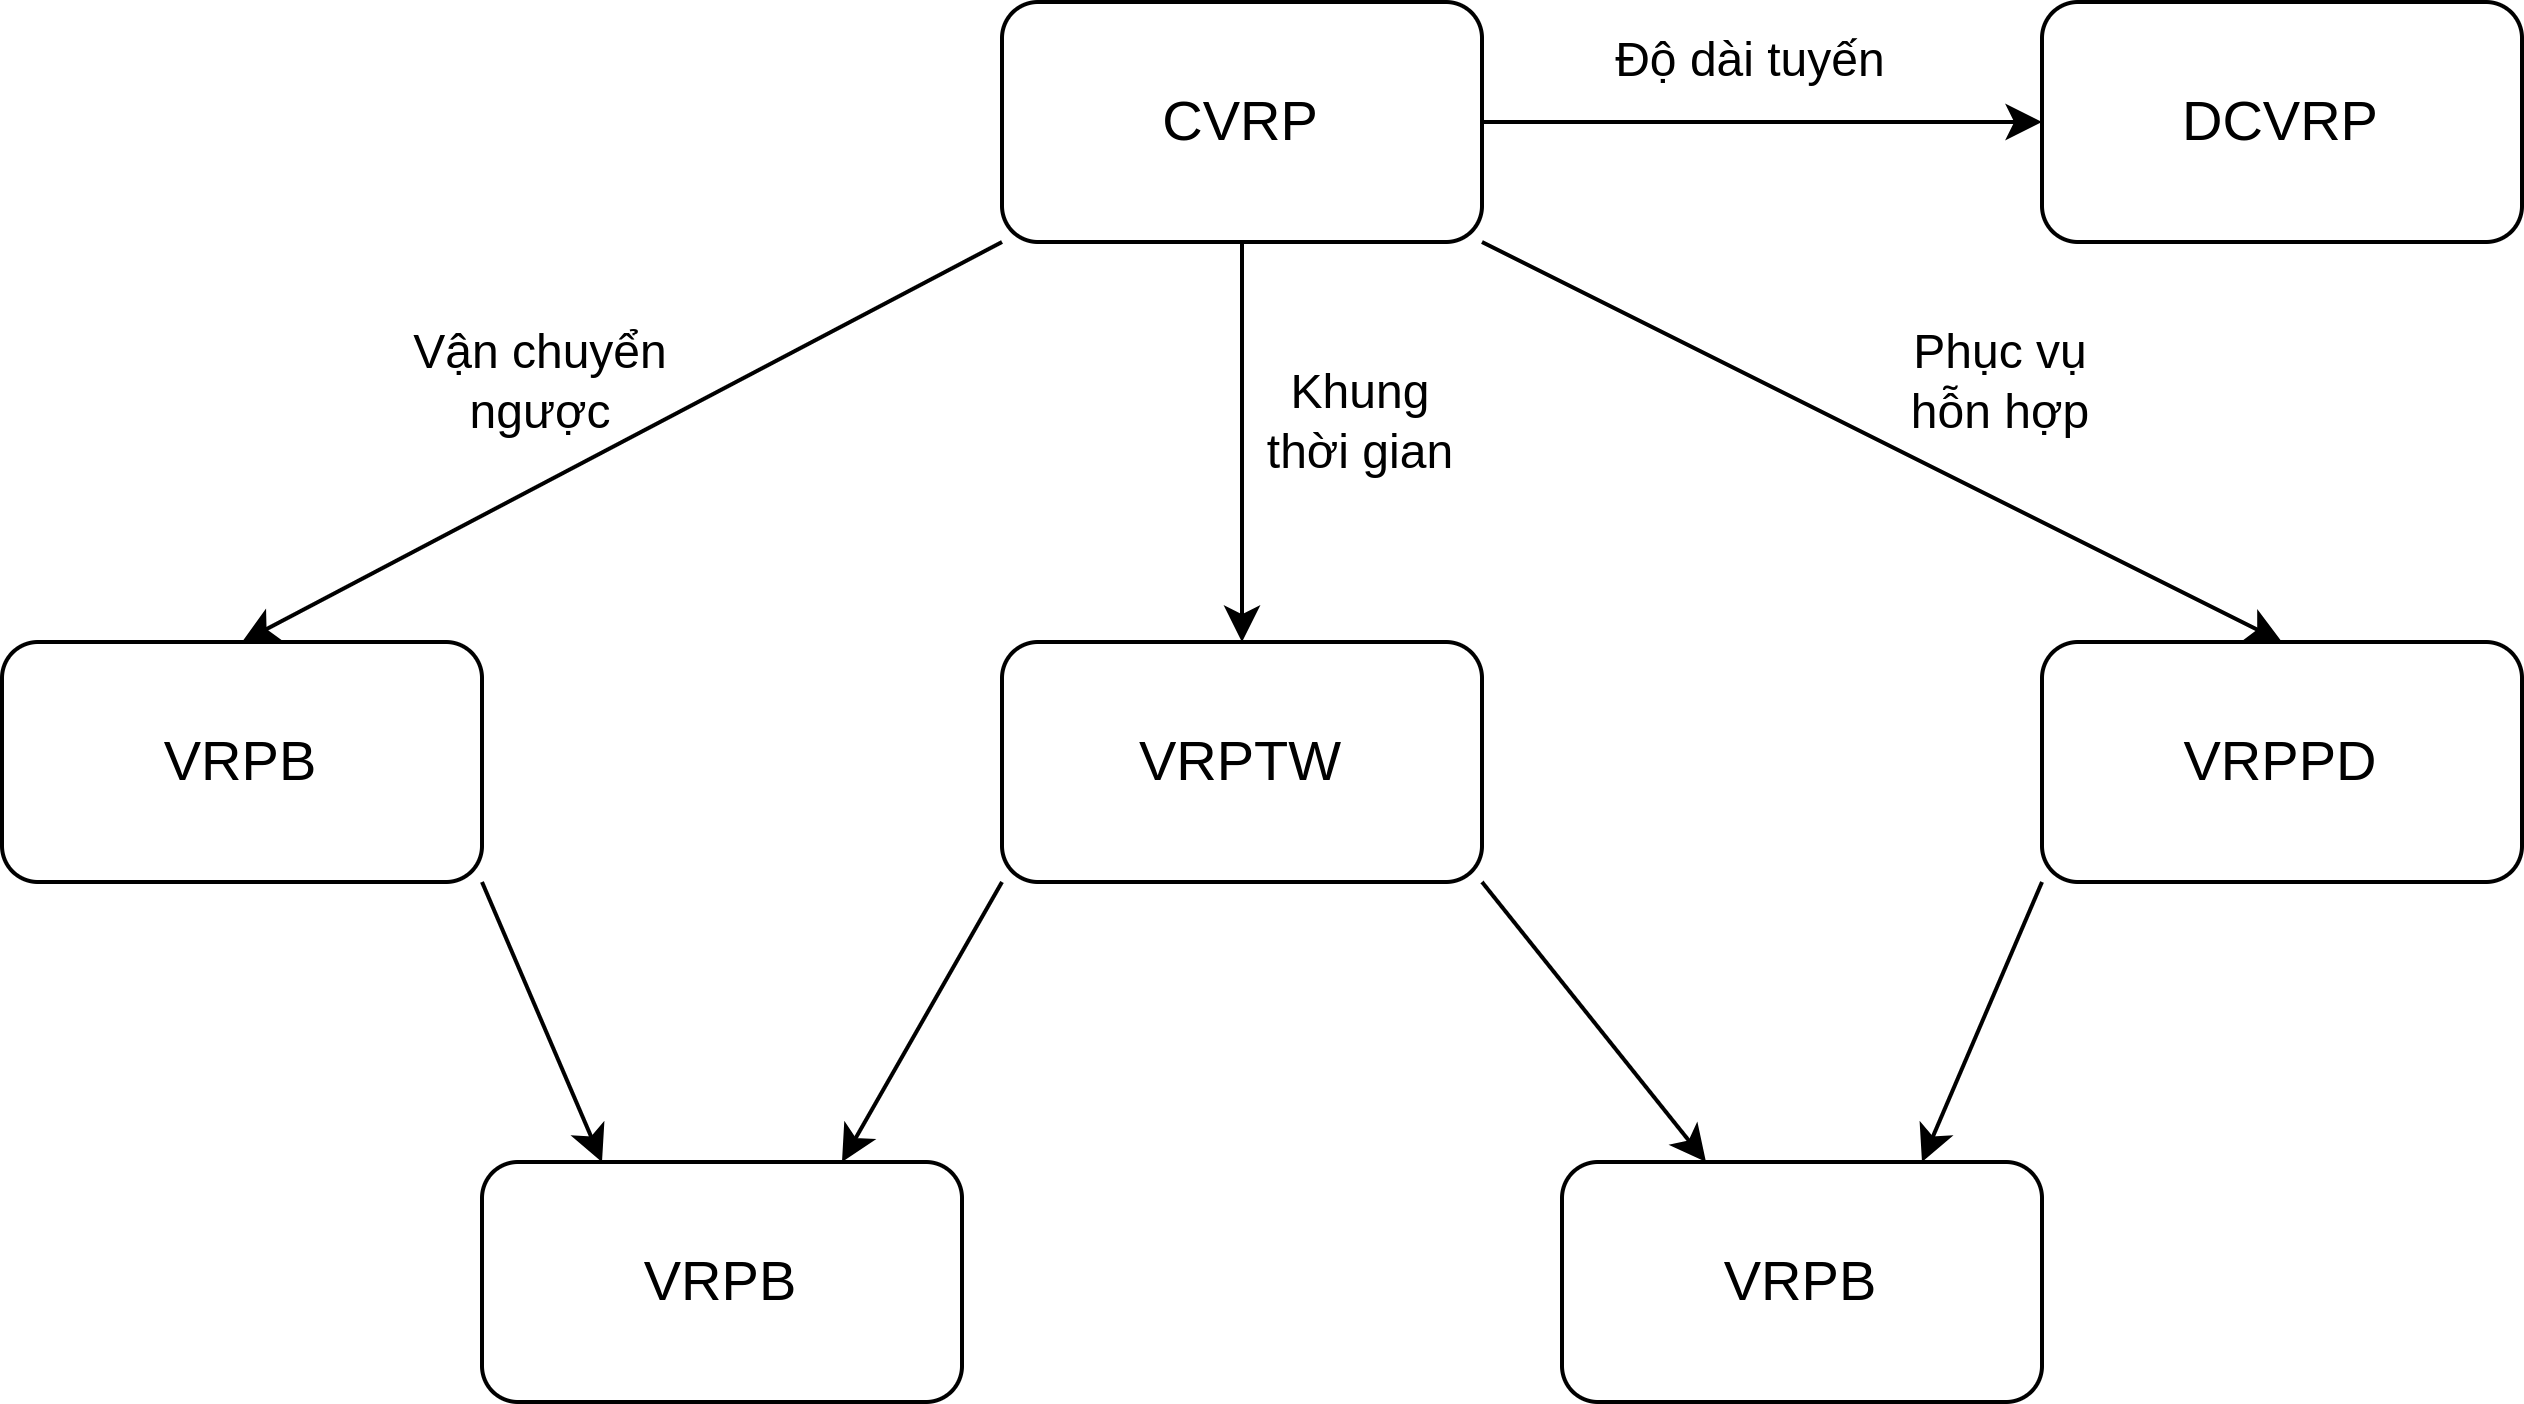
\includegraphics[width=0.8\textwidth]{figures/vrp.png} 
        \caption{Các bài toán, biến thể của VRP} % Creates caption underneath graph
        \label{fig:fg_01}
      \end{figure}
\end{frame}


\begin{frame}{Mô hình - Dòng xe}
    \textbf{Công thức dòng xe hai chỉ số }\\
    $x_{ij}$ nhận giá trị bằng $1$ nếu cung $(i, j) \in A$ nằm trong nghiệm tối ưu và $0$ nếu trong trường hợp còn lại.
    \begin{equation} \label{eq:vrp1}
        \text{(VRP1)} \quad \min \sum_{i \in V} \sum_{j \in V} c_{ij} x_{ij}
      \end{equation}
      s.t.
      \begin{flalign}
          \label{ct_vrp1:1}  & \sum_{i \in V} x_{ij} = 1 \quad \forall j \in V \setminus \{0\}, \\
        \label{ct_vrp1:2}  & \sum_{j \in V} x_{ij} = 1 \quad \forall i \in V \setminus \{0\}, \\
        \label{ct_vrp1:3}  & \sum_{i \in V} x_{i0} = K,
    \end{flalign}
\end{frame}

\begin{frame}{Mô hình - Dòng xe}
    \begin{flalign}
        \label{ct_vrp1:4}  & \sum_{j \in V} x_{0j} = K, \\
        \label{ct_vrp1:5}  & \sum_{i \notin  S} \sum_{j \in S} x_{ij} \geq r(S) \quad \forall S \subseteq V \setminus \{0\}, S \neq \emptyset, \\
        \label{ct_vrp1:6}  & x_{ij} \in \{0,1\} \quad \forall i,j \in V.
    \end{flalign}
\end{frame}

\begin{frame}{Mô hình - VRPTW}
    \textbf{Công thức dòng xe ba chỉ số }\\
    $x_{ijk}$ nhận giá trị 1 nếu xe $k$ đi trực tiếp từ nút $i$ tới nút $j$ và 0 nếu ngược lại.
    \begin{equation} \label{eq1}
        \min \sum_{k \in K} \sum_{(i,j) \in A} c_{ij} x_{ijk}
    \end{equation}
    s.t.
    \begin{flalign}
        \label{ct:1}  & \sum_{k \in K} \sum_{j \in \Delta^+(i)} x_{ijk} = 1 \quad \forall i \in N, \\
        \label{ct:2}  & \sum_{j \in \Delta^+(0)} x_{0jk} = 1 \quad \forall k \in K,                   \\
        \label{ct:3}  & \sum_{i \in \Delta^-(j)} x_{ijk} -  \sum_{i \in \Delta^+(j)} x_{jik} = 0 \quad \forall k \in K, j \in N,
    \end{flalign}
\end{frame}

\begin{frame}
    \begin{flalign}
        \label{ct:4}  & \sum_{i \in \Delta^-(n+1)} x_{i,n+1,k} = 1 \quad \forall k \in K, \\
        \label{ct:5}  & x_{ijk} (w_{ik} + s_i + t_{ij} - w_{jk}) \leq 0 \quad \forall k \in K, (i,j) \in A, \\
        \label{ct:6}  & a_i \sum_{j \in \Delta^+(i)} x_{ijk} \leq w_{ik} \leq b_i \sum_{j \in \Delta^+(i)} x_{ijk} \quad \forall k \in K, i \in N, \\
        \label{ct:7}  & E \leq w_{ik} \leq L \quad \forall k \in K, i \in \{0, n+1\}, \\
        \label{ct:8}  & \sum_{i \in N} d_i \sum_{j \in \Delta^+(i)} x_{ijk} \leq C \quad \forall k \in K, \\
        \label{ct:9}  & x_{ijk} \geq 0 \quad \forall k \in K, (i,j) \in A, \\
        \label{ct:10} & x_{ijk} \in \{0,1\} \quad \forall k \in K, (i,j) \in A.
    \end{flalign}
\end{frame}

\section{Phương pháp}
\begin{frame}{Phương pháp - Thuật toán chính xác}
  \begin{itemize}
    \item Phương pháp nhánh-cận
    \item Quy hoạch động
    \item Mô hình dựa trên dòng xe 
    \item Mô hình dựa trên dòng hàng
    \item Mô hình phân hoạch tập hợp
  \end{itemize}
\end{frame}

\begin{frame}{Phương pháp - Heuristic cổ điển}
  \begin{itemize}
    \item Thuật toán tiết kiệm
    \item Phân cụm trước, định tuyến sau 
    \item Heuristic cải tiến
  \end{itemize}
\end{frame}

\begin{frame}{Phương pháp - Metaheuristics}
  \begin{itemize}
    \item Tìm kiếm địa phương
    \item Tìm kiếm quần thể 
    \item Cơ chế học
  \end{itemize}
\end{frame}



\section{Tìm kiếm lân cận}
\begin{frame}{Tìm kiếm lân cận}
  \begin{itemize}
    \item Lân cận
    \item Tối ưu địa phương
    \item Tiêu chí chấp nhận nghiệm
    \item Điều kiện dừng
  \end{itemize}
\end{frame}

\begin{frame}{Tìm kiếm lân cận rộng}
  \begin{figure}[H] % places figure environment here   
    \centering % Centers Graphic
    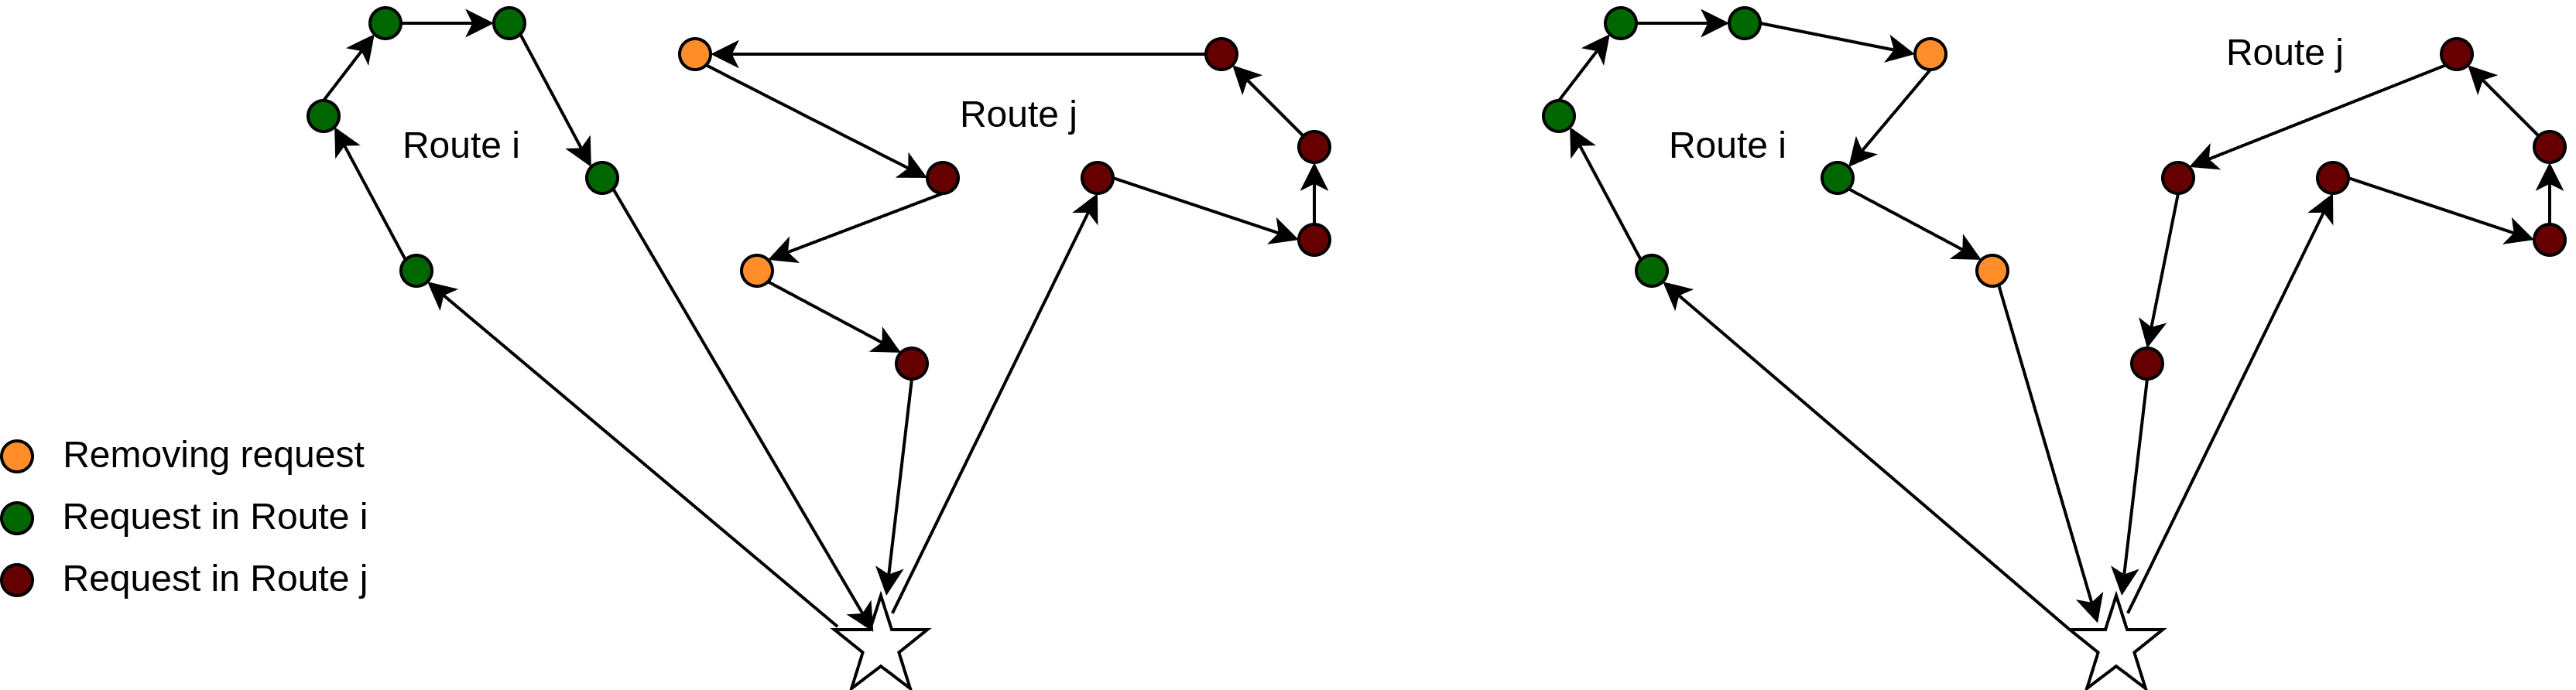
\includegraphics[width=0.9\textwidth]{figures/ALNS-paradim.png} 
    % \includesvg[scale=1]{figures/core-object}
    \caption{Lược đồ LNS} 
    \label{fig:lns_paradim}
  \end{figure}  
\end{frame}

\begin{frame}{Tìm kiếm lân cận rộng (\textit{LNS})}
  \begin{figure}[H] % places figure environment here   
    \centering % Centers Graphic
    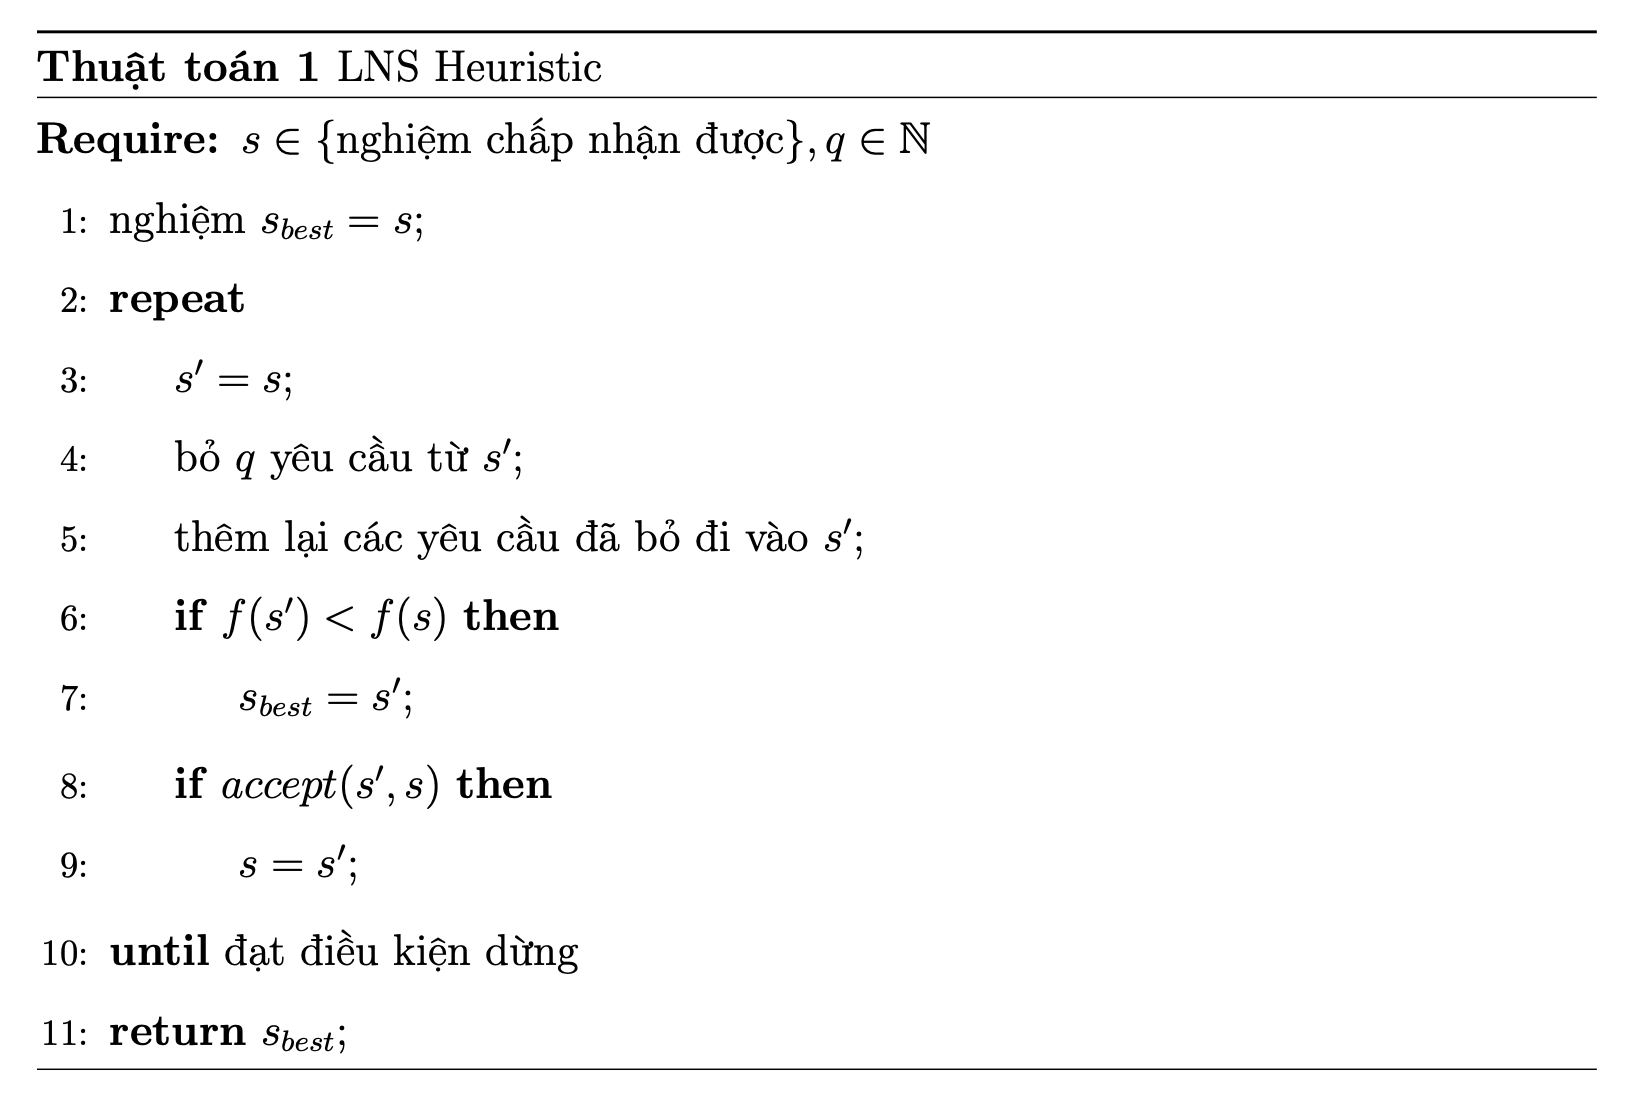
\includegraphics[width=0.8\textwidth]{figures/pr_LNS.png} 
    % \includesvg[scale=1]{figures/core-object}
    \caption{Mã giả LNS} 
    \label{fig:lns_pseudo}
  \end{figure} 
\end{frame}

\begin{frame}{LNS - Thuật toán hủy}
  % \begin{itemize}
  %   \item Xóa yêu cầu tệ nhất
  %   \item Xóa ngẫu nhiên
  %   \item Thuật toán xóa Shaw
  %   \item Thuật toán xóa tuyến tệ
  % \end{itemize}
  \begin{block}{Xóa yêu cầu tệ nhất}
  \end{block}
  \begin{block}{Xóa ngẫu nhiên}
  \end{block}
  \begin{block}{Thuật toán xóa Shaw}
  \end{block}
  \begin{block}{ Thuật toán xóa tuyến tệ}
  \end{block}
\end{frame}

\begin{frame}{LNS - Thuật toán hủy}
  \begin{block}{Xóa yêu cầu tệ nhất}
    \begin{itemize}
      \item Mảng $L$: sắp xếp các yêu cầu theo thứ tự giảm dần của chi phí (sau khi bỏ đi yêu cầu đó).
      \item Chọn một số ngẫu nhiên $y \in (0,1)$.
      \item Xóa yêu cầu $r = L[y^p|L|]$.
    \end{itemize}
  \end{block}
\end{frame}

\begin{frame}{LNS - Thuật toán hủy}
  \begin{block}{Xóa tuyến tệ nhất}
    Chi phí trung bình trên mỗi yêu cầu với nhiễu
    \begin{equation}
      \label{eq:destroy_route}
      \text{avg\_cost}(r, s) = \frac{\text{cost}(r, s)}{\text{size}(r)-1} + \lambda \phi d_{max}
    \end{equation}
    với $r$ là tuyến được chọn, $\text{cost}(r,s)$ là chi phí của tuyến $r$ trong nghiệm $s$, $\text{size}(r)$ là số phần tử của tuyến $r$, $\lambda$ là hệ số nhiễu, $\phi$ là một số ngẫu nhiên trong khoảng $(0,1)$, $d_{max}$ là khoảng cách lớn nhất trong tập yêu cầu.
    
    Xóa đi tuyến có chi phí trung bình trên mỗi yêu cầu lớn nhất và có số yêu cầu nhỏ hơn số yêu cầu trung bình trên mỗi tuyến (với một ngưỡng nhất định).
  \end{block}
\end{frame}

\begin{frame}{LNS - Thuật toán hủy}
  \begin{block}{Phương pháp xóa Shaw}
    Chỉ số độ tương đồng 
    \begin{equation}
      \label{eq:shaw_related}
      R(i,j) = \varphi d_{ij} + \chi |t_{i}-t_{j}| + \psi|l_i - l_j|
    \end{equation}
    với $d_{ij}$ là khoảng cách từ $i$ tới $j$, $t_i$ là thời gian khi đến địa điểm $i$, $l_i$ là tải của xe tại $i$.
  \end{block}
\end{frame}

\begin{frame}{LNS - Thuật toán hủy}
  \begin{figure}[H] % places figure environment here   
    \centering % Centers Graphic
    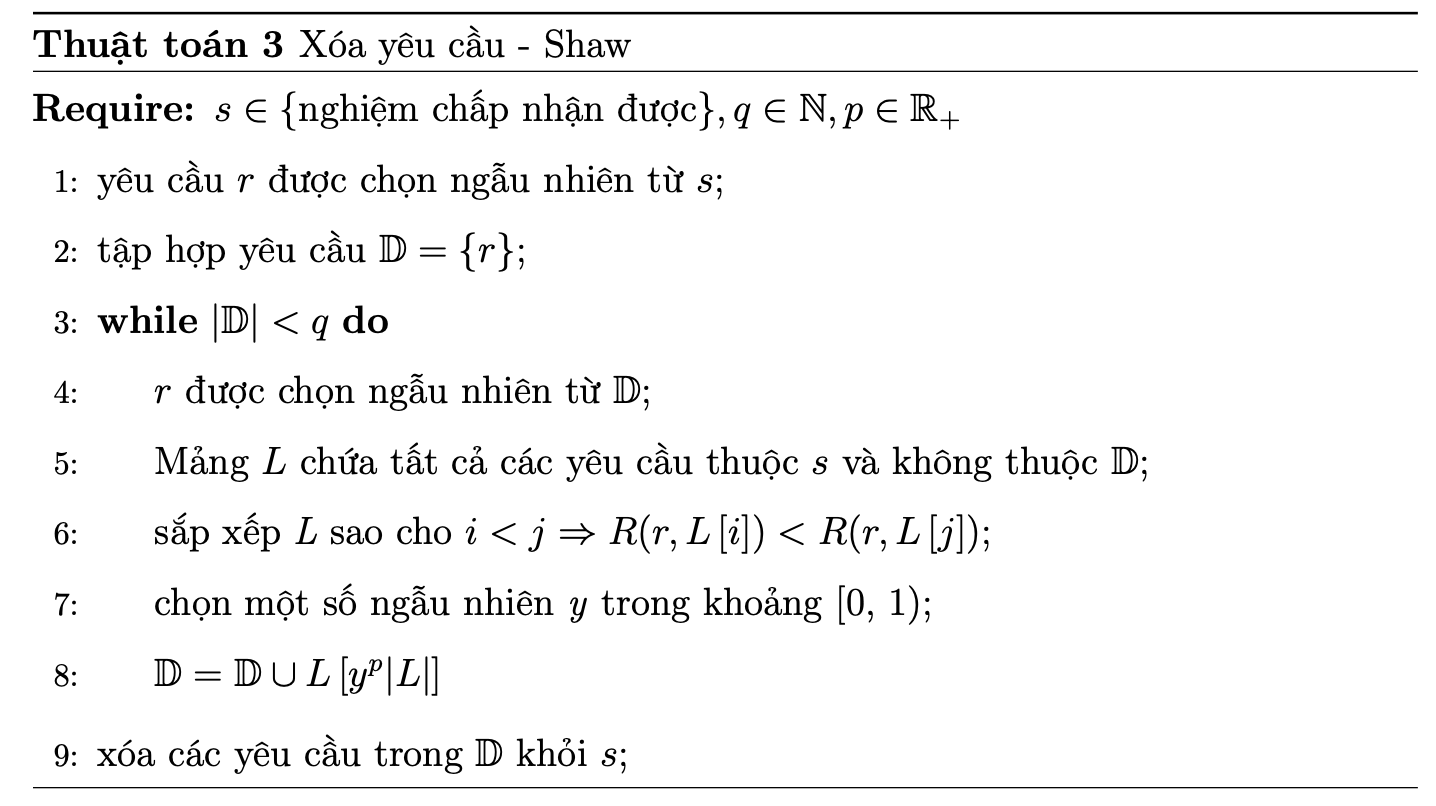
\includegraphics[width=1\textwidth]{figures/des_shaw.png} 
    % \includesvg[scale=1]{figures/core-object}
    \caption{Thuật toán xóa Shaw} 
    \label{fig:shaw_pseudo}
  \end{figure} 
\end{frame}

\begin{frame}{LNS - Thuật toán sửa}
  % \begin{itemize}
  %   \item Chèn yêu cầu tham lam (với nhiễu)
  %   \item Heuristic hối tiếc
  % \end{itemize}  
  \begin{block}{Chèn yêu cầu tham lam (với nhiễu)}
  \end{block}
  \begin{block}{Heuristic hối tiếc}
  \end{block}
\end{frame}

\begin{frame}{LNS - Thuật toán sửa}
  \begin{block}{Chèn yêu cầu tham lam}
    \begin{itemize}
      \item Khi chèn thêm yêu cầu $u$ và giữa hai yêu cầu $i$ và $j$ trong tuyến $k$ thì chi phí tăng thêm là $\Delta f_{u, i, j, k} = d_{iu} + d_{uj} - d_{ij}$.
      \item Chèn thêm yêu cầu vào vị trí làm tăng ít chi phí nhất.
      \item Có thể thêm nhiễu vào hàm tăng chi phí.
      \begin{equation}
        \Delta f_{u, i, j, k} := \Delta f_{u, i, j, k} + \lambda p d_{\text{max}}
      \end{equation}
      với $d_{\text{max}}$ là khoảng cách lớn nhất giữa hai yêu cầu, $p$ là một số ngẫu nhiên trong khoảng $(-1,1)$ và $\lambda$ là một hằng số điều khiển.
    \end{itemize}
  \end{block}
\end{frame}

\begin{frame}{LNS - Thuật toán sửa}
  \begin{block}{Heuristic hối tiếc}
    \begin{itemize}
      \item Đặt $x_{ik} \in \{1, ..., m\}$ là biến biểu diễn tuyến đường cho yêu cầu $i$ có chi phí chèn thêm vào thấp thứ $k$.
      \item Giá trị \textit{regret} $c_i^* = \Delta f_{i, x_{i2}} - \Delta f_{i, x_{i1}}$.
      \item Chọn ra yêu cầu $i$ thỏa mãn $\max_{i \in V \setminus \{0\}} \{c_i^*\}$ và chèn vào vị trí tương ứng.
      \item Mở rộng regret-k, chọn yêu cầu thỏa mãn
      \begin{equation}
        \max\limits_{i \in V \setminus \{0\} } \{ \sum_{j=1}^k (\Delta f_{i, x_{ij}} - \Delta f_{i, x_{i1}}) \}.
    \end{equation}
    \end{itemize}
  \end{block}
\end{frame}

\begin{frame}{LNS - Tiêu chí chấp nhận nghiệm}
    \begin{block}{Bước ngẫu nhiên - Ramdom Walk}
      Mọi nghiệm $s'$ đều được chấp nhận.
    \end{block}
    \begin{block}{Chấp nhận tham lam - Greedy Acceptance}
      Nghiệm $s'$ được chấp nhận nếu chi phí của nó là nhỏ hơn so với nghiệm hiện tại.
    \end{block}
    \begin{block}{Mô phỏng luyện kim - Simulated Annealing}
      Mọi nghiệm cải thiện $s'$ được chấp nhận. Nếu $c(s') > c(s)$ thì $s'$ được chấp nhận với xác suất $\exp \{ \frac{c(s) - c(s')}{T} \}$ với $T$ là nhiệt độ. Nhiệt độ $T$ giảm sau mỗi vòng lặp với một hệ số $\Phi$.
    \end{block}
\end{frame}

\begin{frame}{LNS - Tiêu chí chấp nhận nghiệm}
  \begin{block}{Chấp nhận với ngưỡng - Threshold Acceptance}
    Nghiệm $s'$ được chấp nhận nếu $c(s') - c(s) < T$ với $T$ là ngưỡng, ngưỡng này được giảm sau mỗi vòng lặp với hệ số $\Phi$.
  \end{block}
  
  \begin{block}{Đại hồng thủy - Great Deluge Algorithm}
    Nghiệm $s'$ được chấp nhận nếu $c(s') < L$ với một ngưỡng $L$, ngưỡng này chỉ giảm nếu nghiệm được chấp nhận và giảm với hệ số $\Phi$.
  \end{block}
\end{frame}

% \begin{frame}{Tìm kiếm lân cận rộng thích ứng (\textit{ALNS})}
%   \begin{figure}[H] % places figure environment here   
%     \centering % Centers Graphic
%     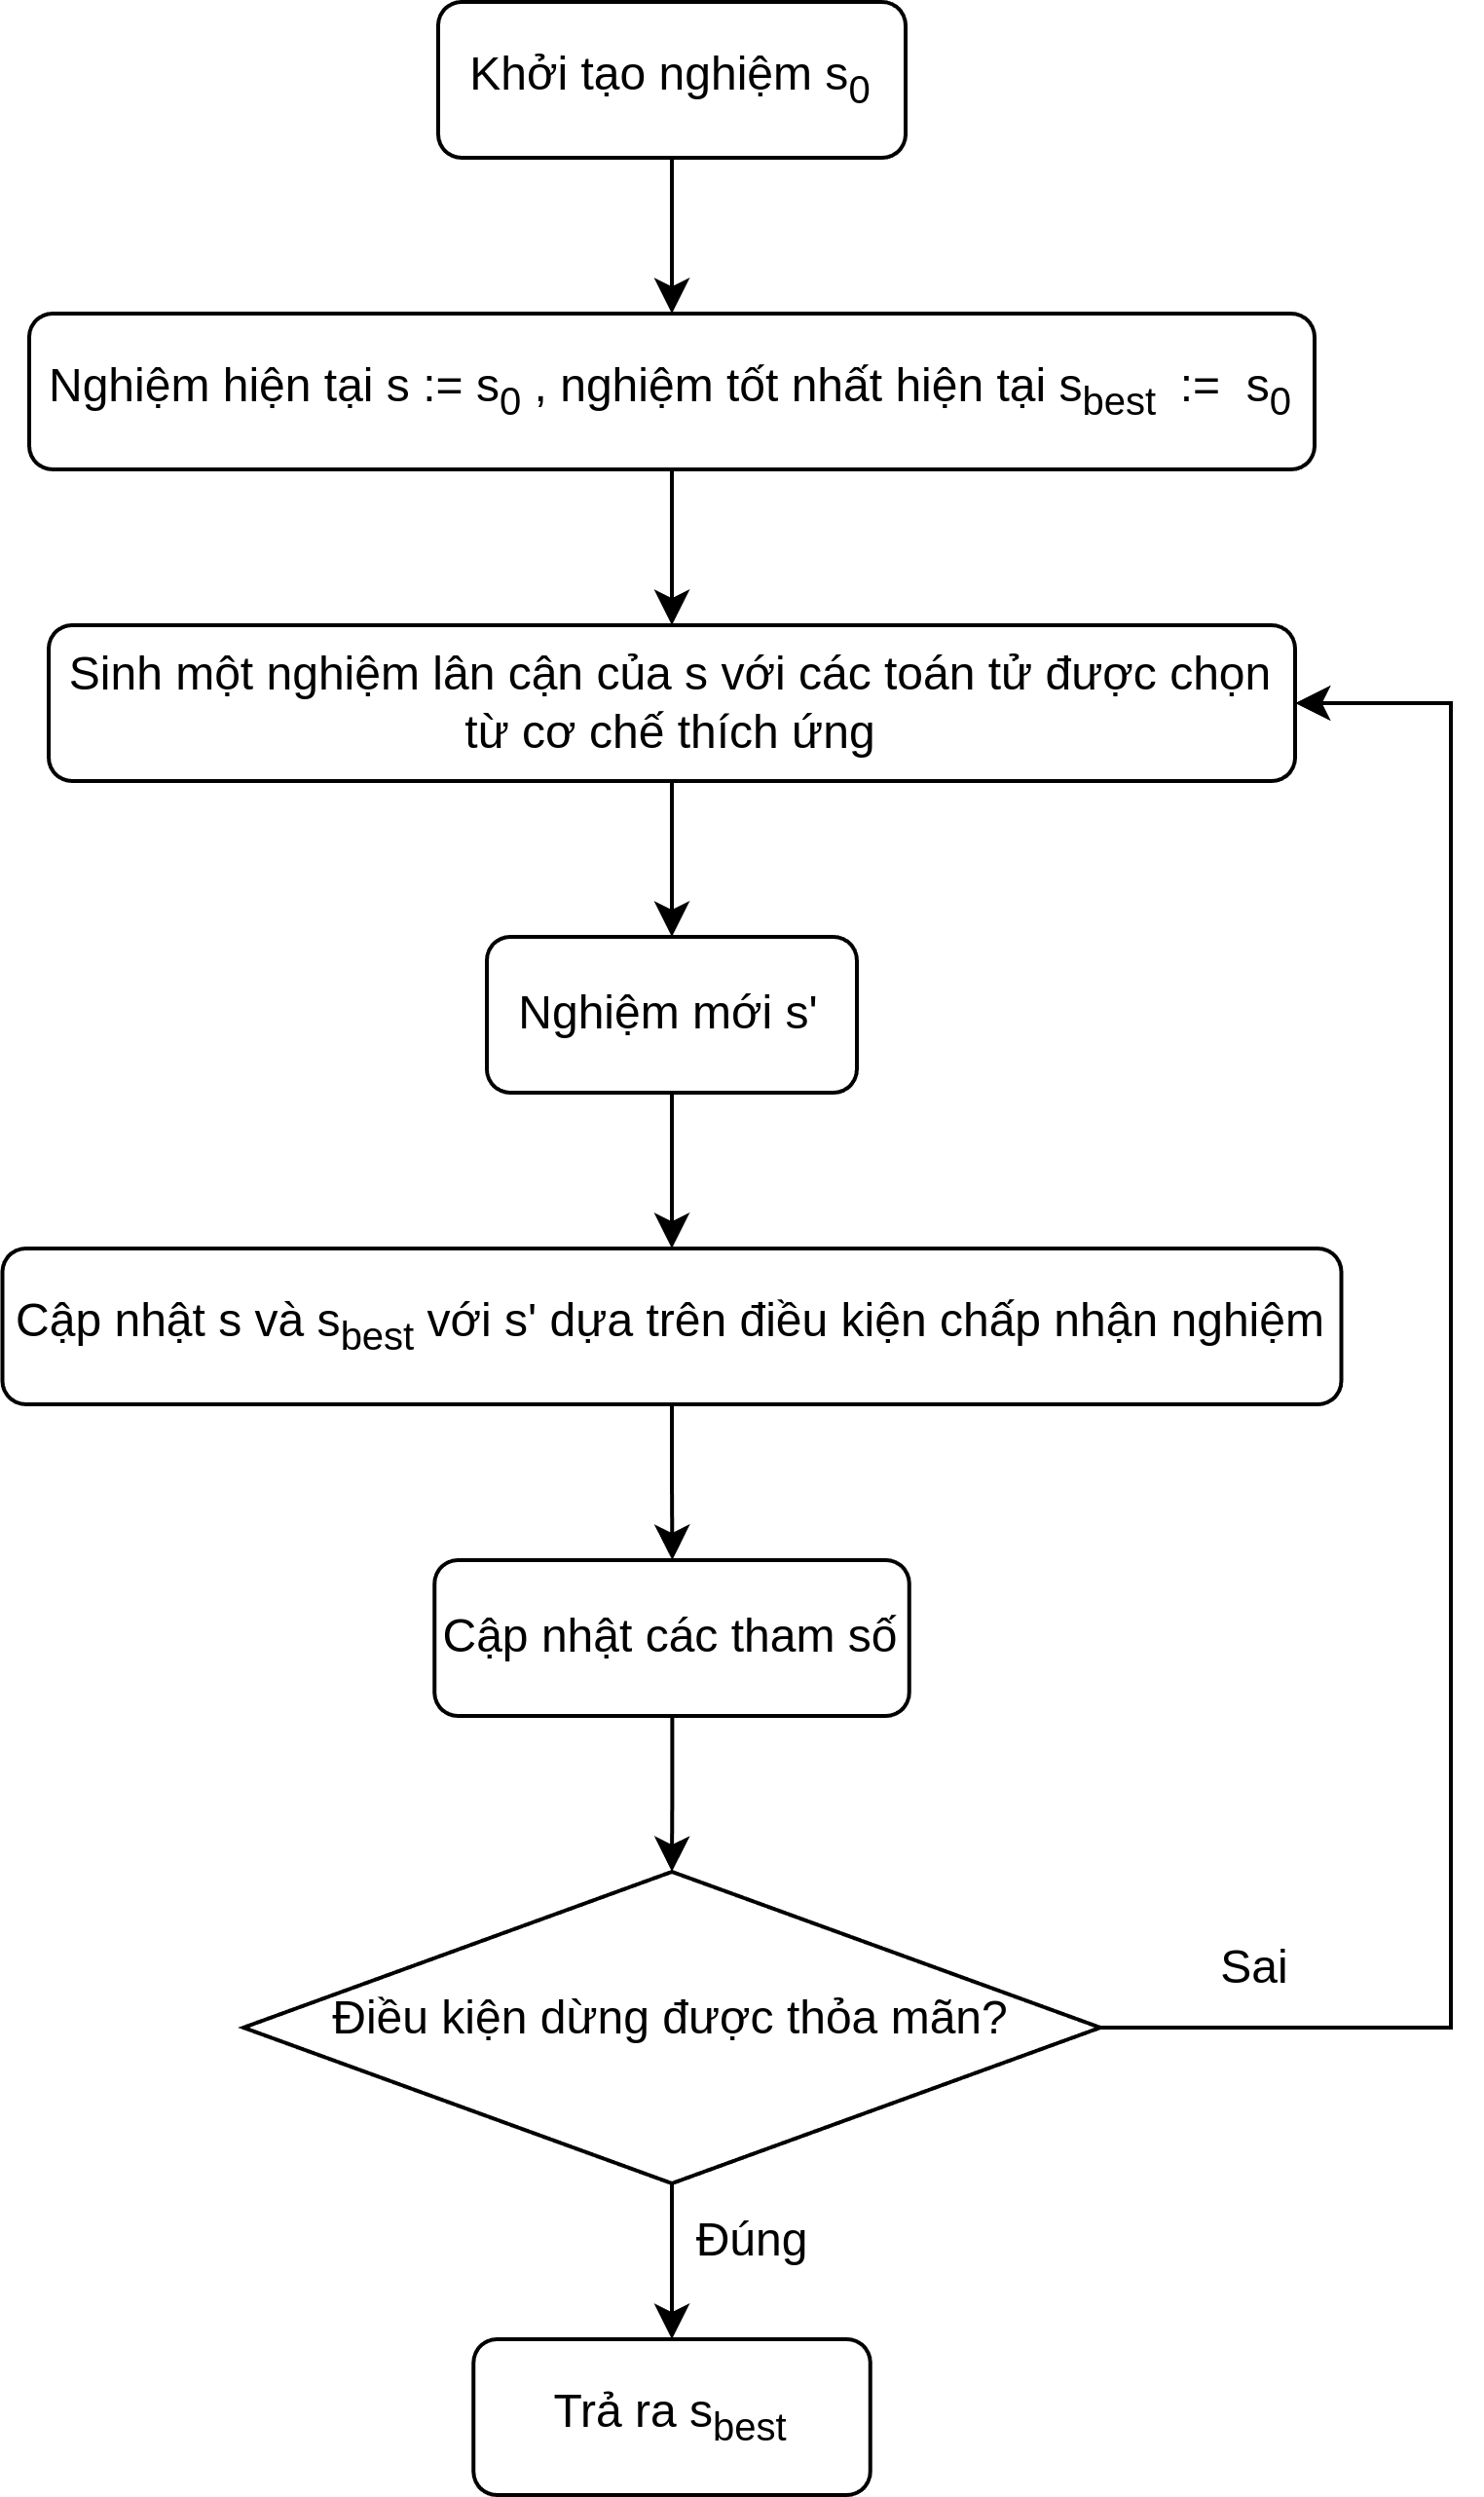
\includegraphics[width=0.3\textwidth]{figures/ALNS-flowchart.png} 
%     % \includesvg[scale=1]{figures/core-object}
%     \caption{Lược đồ chính của ALNS} 
%     % \label{fig:fg_02}
%   \end{figure}
% \end{frame}

\begin{frame}{ALNS - Lựa chọn thuật toán}
  \begin{block}{Lựa chọn thuật toán hủy và thêm lại}
    Gán cho mỗi heuristic một trọng số khác nhau và sử dụng nguyên tắc "bánh xe lựa chọn". Nếu có $k$ heuristic với trọng số $w_i, i \in \{1,...,k\}$, ta chọn heuristic $j$ với xác suất
    \begin{equation}
      \label{eq:select}
      p_j = \frac{w_j}{\sum_{i=1}^k w_i}.
    \end{equation}
  \end{block}
\end{frame}

\begin{frame}{ALNS - Điều chỉnh tham số tự động}
  \begin{itemize}
    \item Trọng số được điều chỉnh mỗi khi có nghiệm mới được chấp nhận.
    \item Mỗi heuristic được gán điểm khác nhau và được điều chỉnh tùy thuộc vào tình huống.
    \item Cập nhật trọng số sau mỗi bước.
  \end{itemize}
\end{frame}

\begin{frame}{ALNS - Điều chỉnh tham số tự động}
  $\omega_{ij}$ là trọng số của heuristic $i$ được sử dụng tại bước $j$ \\
  Khi bước $j$ kết thúc, ta tính toán trọng số cho tất cả heuristic $i$ để sử dụng cho bước thứ $j + 1$
  \begin{equation}
      \omega_{i, j+1} = \omega_{ij}(1-r)+r\frac{\pi_i}{\theta_i}.
  \end{equation} \\
  Trong đó, $\pi_i$ là điểm số của heuristic $i$ được nhận trong bước cuối cùng, $\theta_i$ là số lần ta cố gắng sử dụng heuristic $i$ trong bước thực hiện đó, $r$ là tham số điều khiển.
\end{frame}

\begin{frame}{ALNS - Điều chỉnh tham số tự động}
  Điểm của mỗi heuristic được đặt là $0$ khi bắt đầu và được tăng thêm $\sigma_1, \sigma_2, \sigma_3$ tùy thuộc vào tình huống.
  \begin{itemize}
    \justifying
    \item $\sigma_1$ khi hành động xóa-chèn cuối cùng dẫn đến một nghiệm mới tốt hơn nghiệm tốt nhất toàn cục.
    \item $\sigma_2$ khi hành động xóa-chèn cuối cùng dẫn đến một nghiệm chưa được chấp nhận trước đó, chi phí tốt hơn chi phí của nghiệm hiện tại.
    \item $\sigma_3$ khi hành động xóa-chèn cuối cùng dẫn đến một nghiệm chưa được chấp nhận trước đó, chi phí của nghiệm mới tệ hơn chi phí của nghiệm hiện tại nhưng thỏa mãn điều kiện chấp nhận nghiệm.
  \end{itemize}
\end{frame}

\begin{frame}{ALNS - B-ALNS}
  \begin{block}{B-ALNS}
    Thêm nhiễu khi điều chỉnh tham số tự động. Giả sử sau $m$ vòng lặp, chúng ta mới lại có một nghiệm được chấp nhận từ lần cuối cùng nghiệm được chấp nhận.
    \begin{equation}
      \label{eq:boost_adaptive_weight}
      \omega_{i, j+1} = \omega_{ij}(1-r)+r\frac{\pi_i} {\theta_i} + \alpha \beta (1 - e^{-\gamma m})
    \end{equation}
    với $\alpha$ (có thể âm hoặc dương) và $\gamma$ (dương) là các tham số điều khiển, $\beta$ là một số ngẫu nhiên trong khoảng $(0,1)$.
  \end{block}
\end{frame}

% \begin{frame}{ALNS - Số lượng yêu cầu bỏ đi, thêm lại}
%   \begin{itemize}
%     \item Bỏ đi một số lượng yêu cầu cố định. 
%     \item Chọn ngẫu nhiên số lượng bỏ đi trong một khoảng nhất định.
%   \end{itemize}
% \end{frame}



\section{Ứng dụng ALNS}
\begin{frame}{Ứng dụng}
  \begin{figure}[H] % places figure environment here   
    \centering % Centers Graphic
    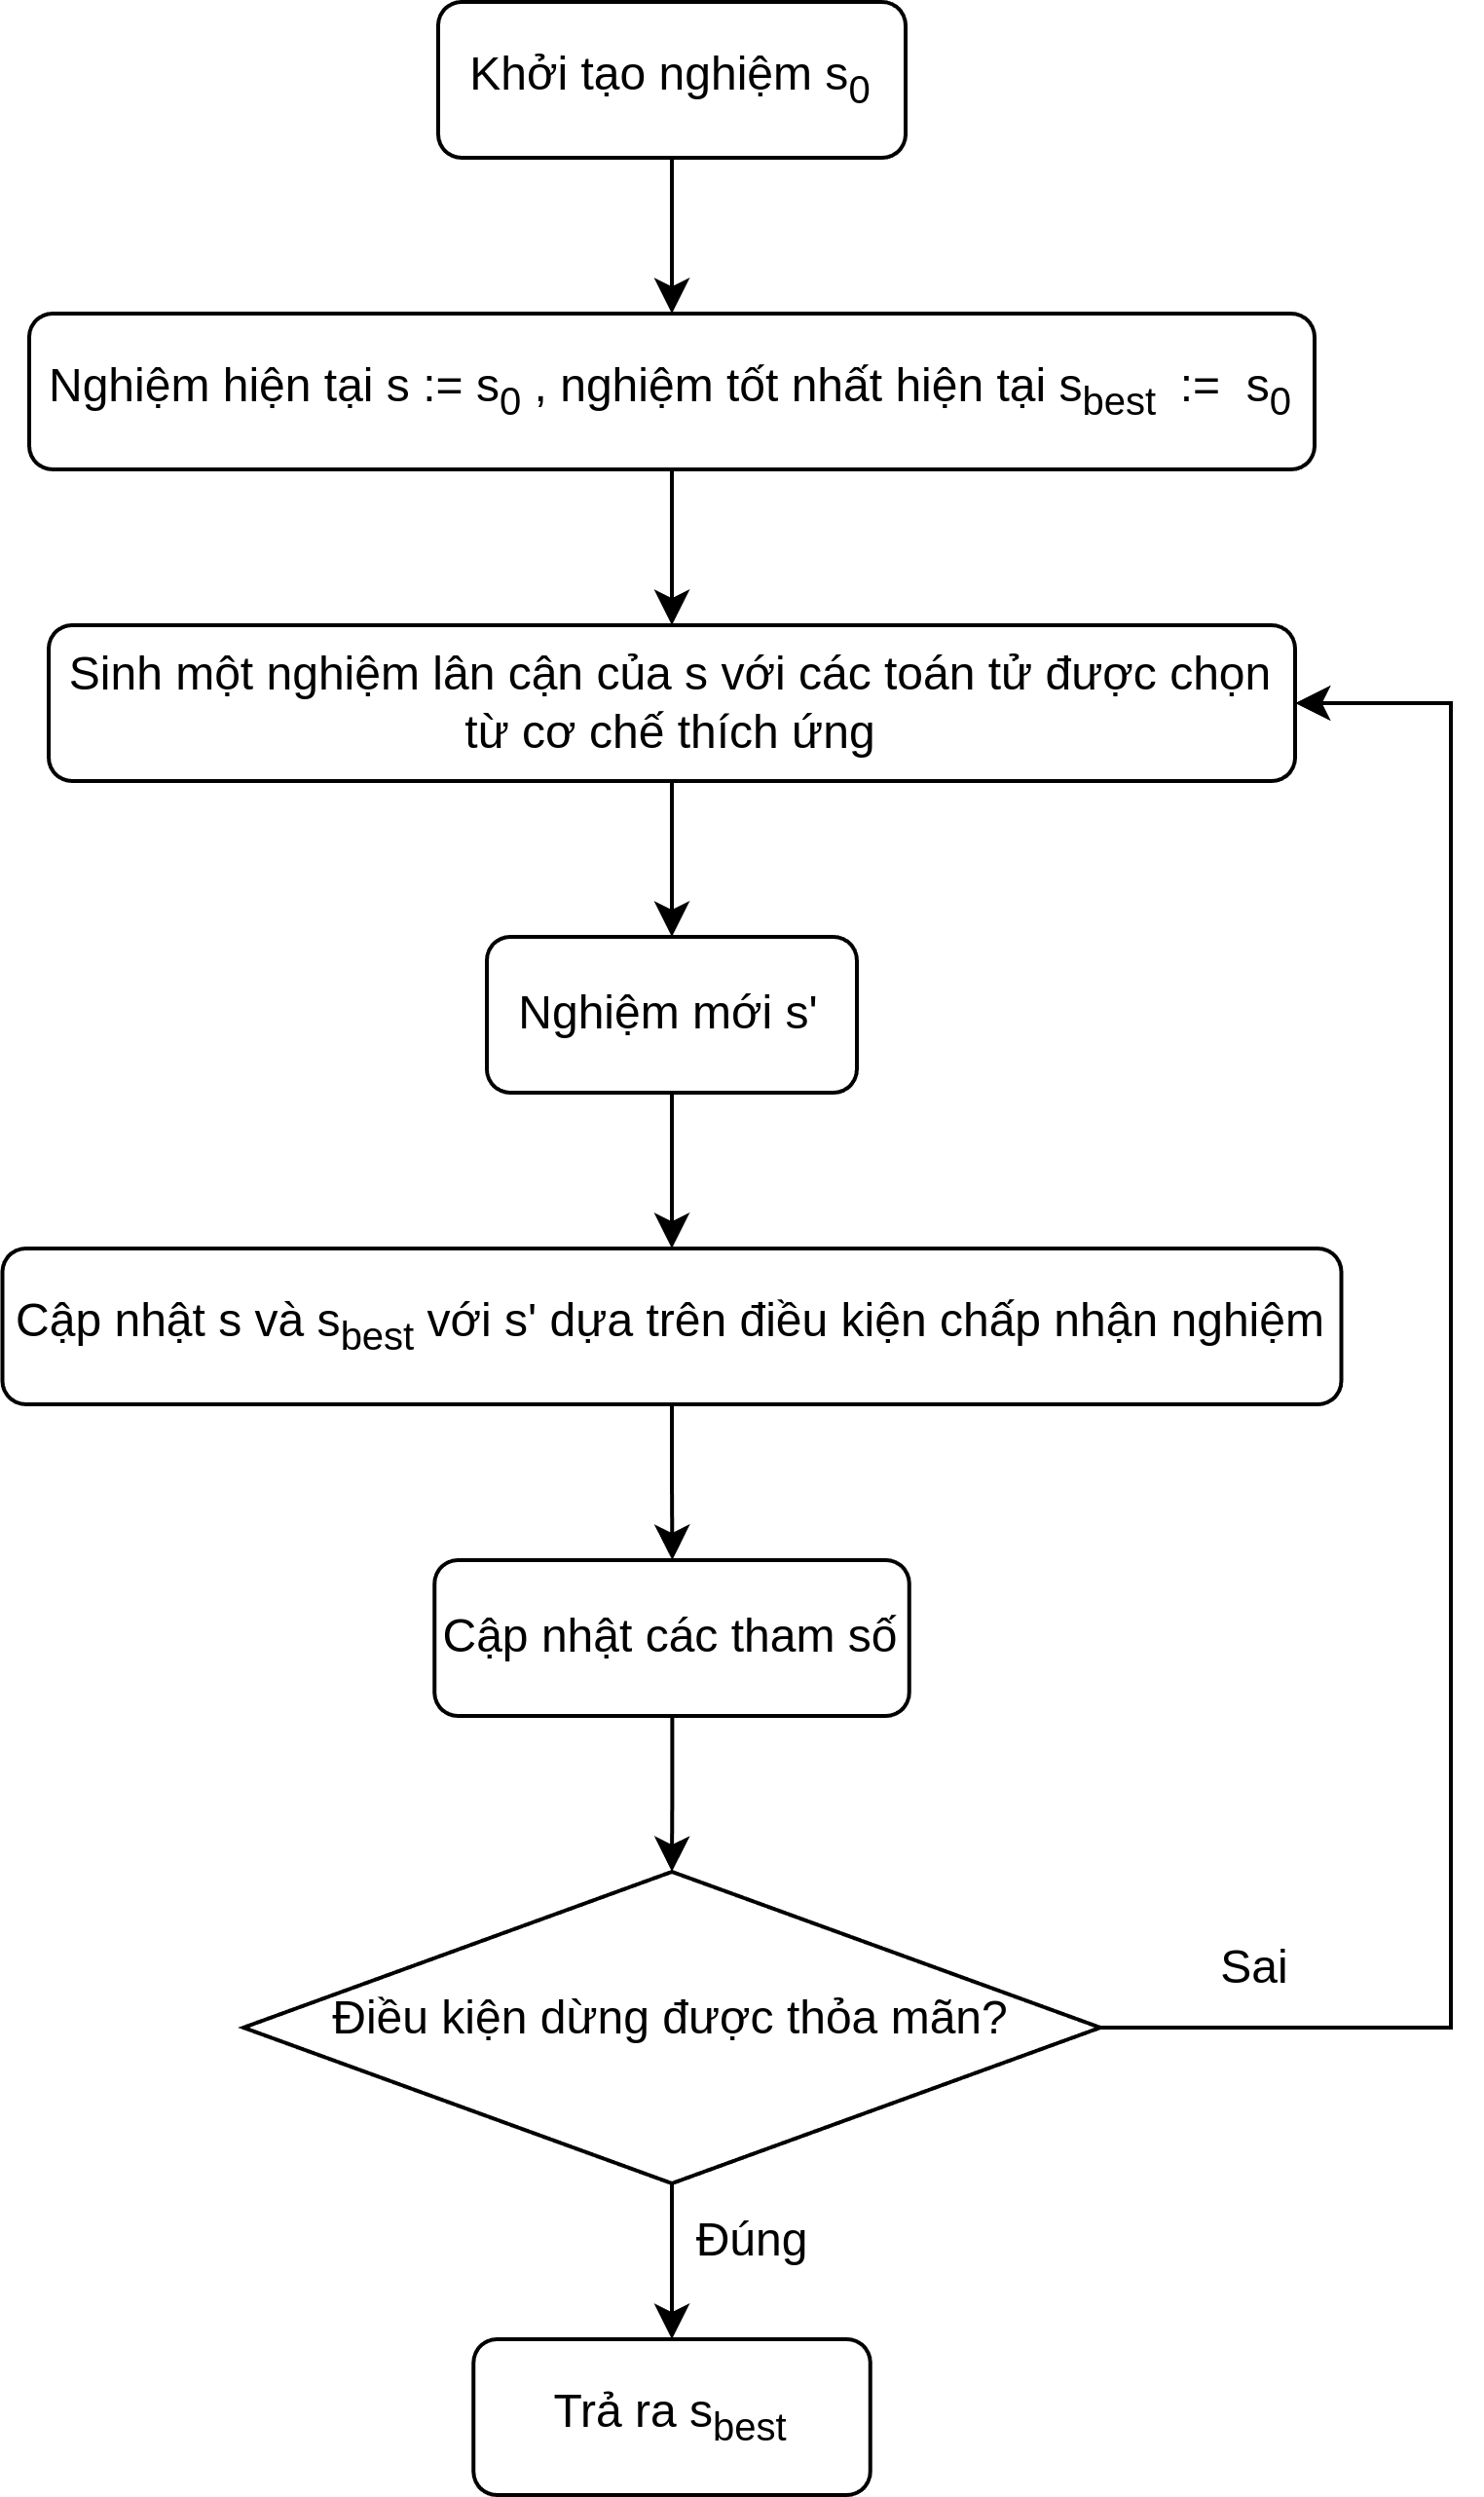
\includegraphics[width=0.3\textwidth]{figures/ALNS-flowchart.png} 
    \caption{Lược đồ chính của ALNS} 
  \end{figure}
\end{frame}

\begin{frame}{Ứng dụng - Các lớp chính}
  \begin{figure}[H] % places figure environment here   
    \centering % Centers Graphic
    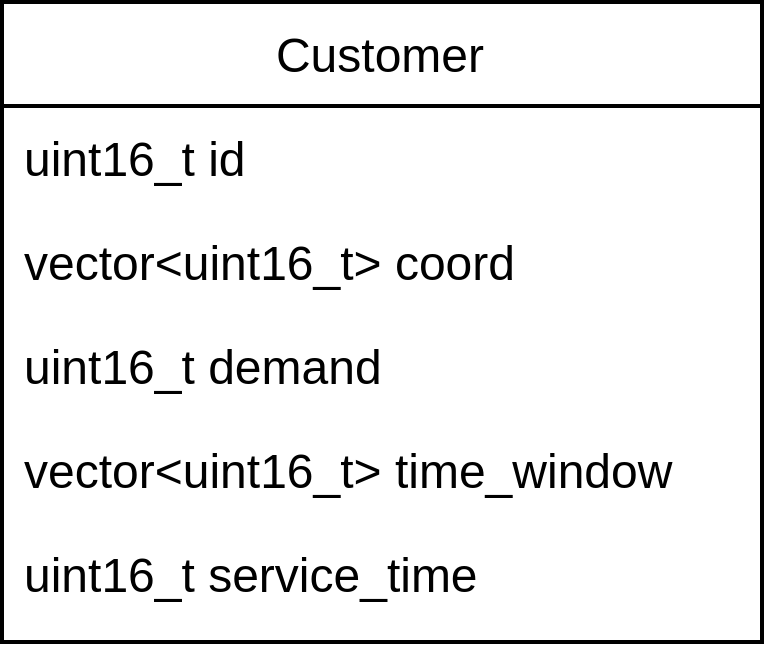
\includegraphics[width=0.35\textwidth]{figures/Customer.png}
    % \includesvg[scale=1]{figures/core-object}
    \caption{Lớp thuộc tính của khách hàng}
    \label{fig:fg_02}
  \end{figure}
\end{frame}

\begin{frame}{Ứng dụng - Các lớp chính}
  \begin{figure}[H] % places figure environment here   
    \centering % Centers Graphic
    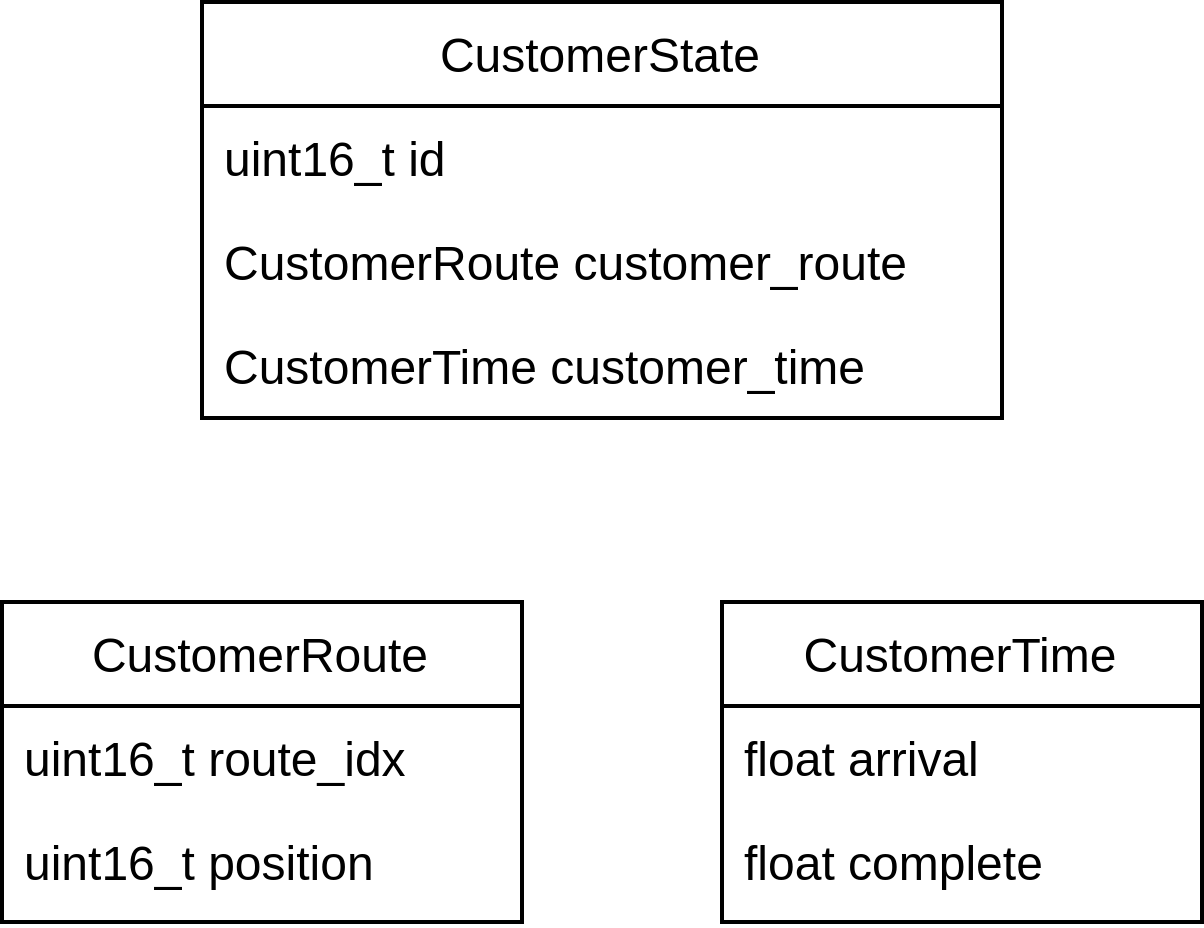
\includegraphics[width=0.6\textwidth]{figures/CustomerState.png}
    % \includesvg[scale=1]{figures/core-object}
    \caption{Lớp trạng thái của khách hàng}
    \label{fig:fg_03}
  \end{figure}
\end{frame}

\begin{frame}{Ứng dụng - Các lớp chính}
  \begin{figure}[H] % places figure environment here   
    \centering % Centers Graphic
    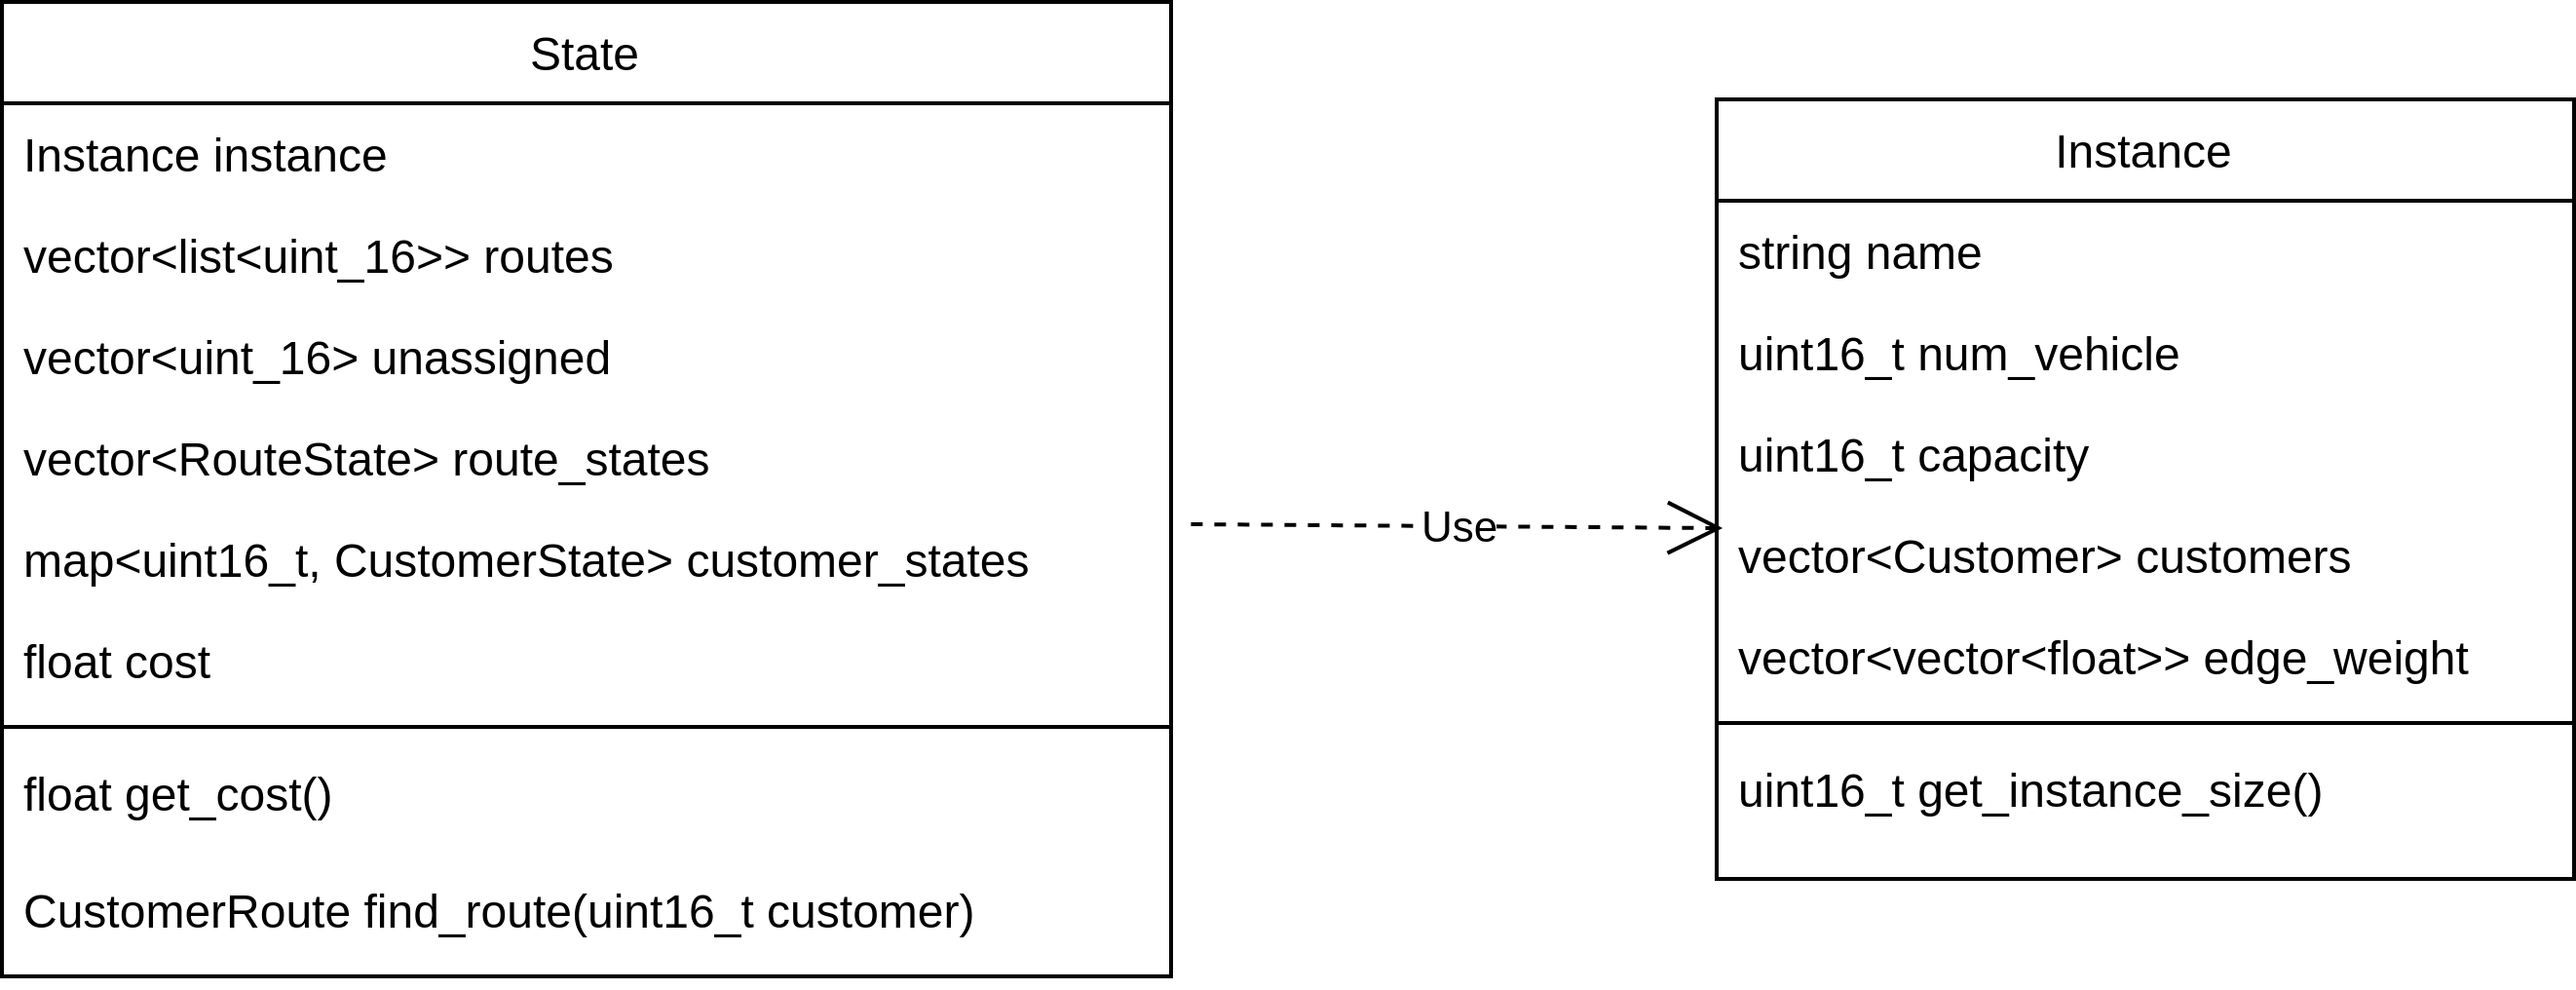
\includegraphics[width=1\textwidth]{figures/core-object.png}
    % \includesvg[scale=1]{figures/core-object}
    \caption{Lớp trạng thái của hệ}
    \label{fig:fg_04}
  \end{figure}
\end{frame}

\begin{frame}{Ứng dụng - Triển khai thuật toán}
  Chương trình được chia làm ba giai đoạn \textit{Tiền xử lý}, \textit{Chương trình chính}, \textit{Đo đạc}.
\begin{itemize}
	\item \textit{Tiền xử lý}: đọc cấu hình, tính toán ma trận khoảng cách, lưu trữ vào các tệp. 
	\item \textit{Chương trình chính}: triển khai ALNS.
	\item \textit{Đo đạc}: phân tích logs, tính toán các độ đo.
\end{itemize}
\end{frame}

\section{Thực nghiệm}
\begin{frame}{Thực nghiệm - Phân loại cấu hình}
  \begin{figure}
    \centering
    \subfloat[Lớp C]{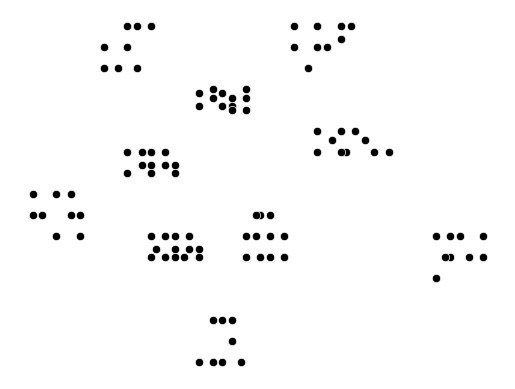
\includegraphics[width=0.3\linewidth]{figures/cls_c.png}}\quad
    \subfloat[Lớp R]{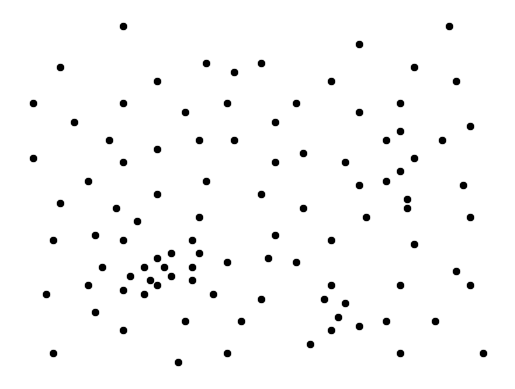
\includegraphics[width=0.3\linewidth]{figures/cls_r.png}}\quad
    \subfloat[Lớp RC]{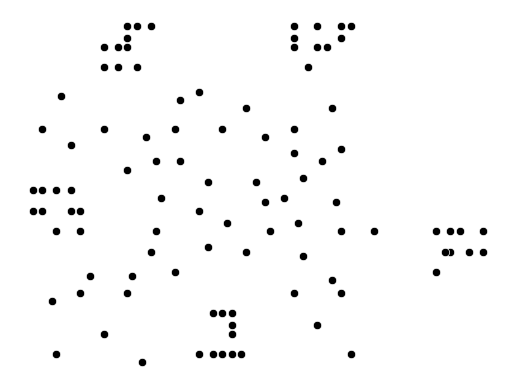
\includegraphics[width=0.3\linewidth]{figures/cls_rc.png}}
  \caption{Lớp các cấu hình}
  \label{fig:perf_ct_c1}
  \end{figure}
\end{frame}

\begin{frame}{Thực nghiệm - Phân loại cấu hình}
  \begin{figure}
    \centering
    \subfloat[Lớp C]{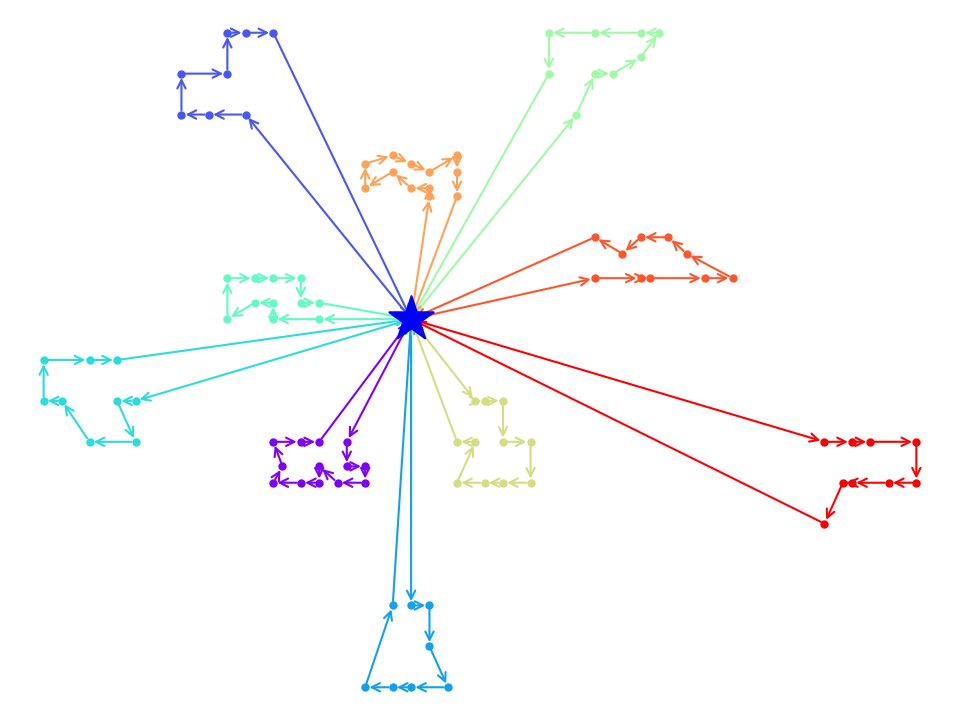
\includegraphics[width=0.3\linewidth]{figures/routes_c101.png}}\quad
    \subfloat[Lớp R]{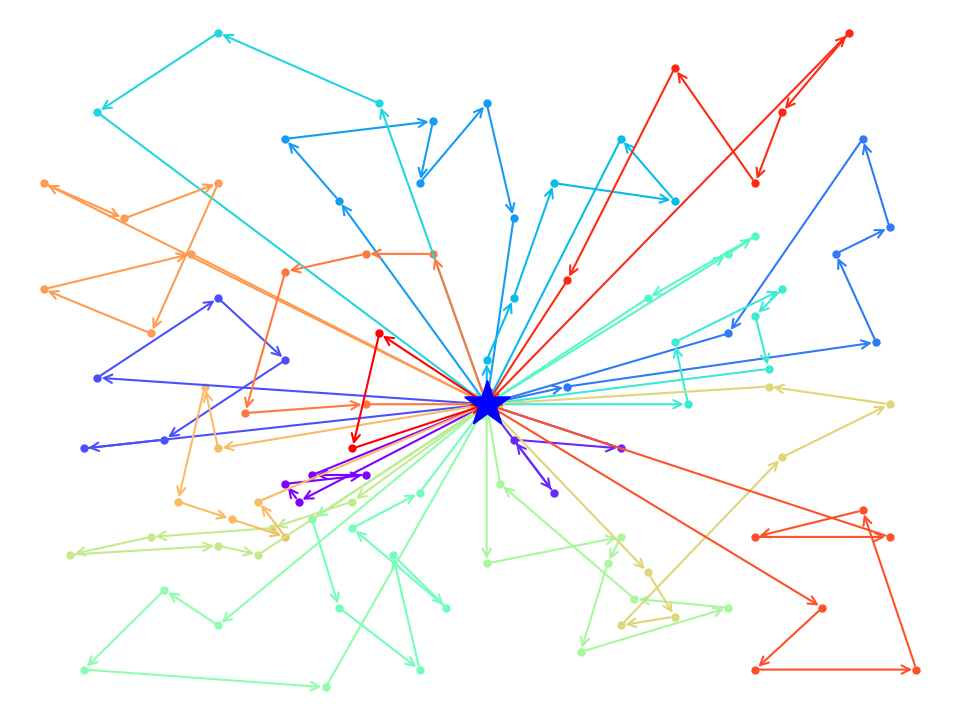
\includegraphics[width=0.3\linewidth]{figures/routes_r101.png}}\quad
    \subfloat[Lớp RC]{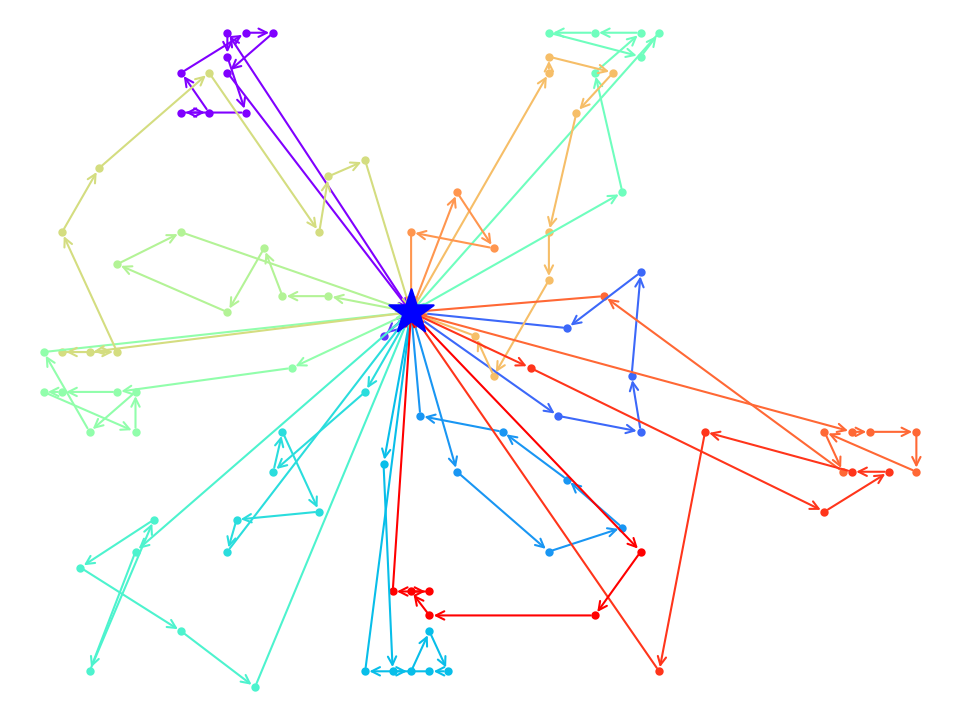
\includegraphics[width=0.3\linewidth]{figures/routes_rc101.png}}
    \caption{Minh họa lời giải cho các lớp cấu hình}
  \end{figure}
\end{frame}

\begin{frame}{Thực nghiệm}
  \begin{block}{Định dạng cấu hình Solomon}
    \begin{itemize}
      \item Tên cấu hình
      \item Số xe được sử dụng
      \item Tải trọng của mỗi xe
      \item ID của yêu cầu
      \item Tọa độ các yêu cầu
      \item Nhu cầu (về tải) của mỗi yêu cầu
      \item Khung thời gian của mỗi yêu cầu
      \item Thời gian phục vụ của mỗi yêu cầu
    \end{itemize}
  \end{block}
\end{frame}

\begin{frame}{Thực nghiệm - Tập Solomon}
  \begin{table}
    \begin{tabular}{|c|c|c|c|}
      \hline
      ins & ALNS & best known & gap (\%) \\ \hline
      c1 & 828.38 & 826.70 & 0.20 \\ \hline
      c2 & 589.86 & 587.38 & 0.42 \\ \hline
      r1 & 1,180.36 & 1,173.61 & 0.61 \\ \hline
      r2 & 883.92 & 872.51 & 1.38 \\ \hline
      rc1 & 1,339.14 & 1,334.49 & 0.36 \\ \hline
      rc2 & 1,007.99 & 1,000.68 & 0.74 \\ \hline
    \end{tabular}
    \caption{Kết quả thực nghiệm trên tập Solomon}
  \end{table}
\end{frame}

\begin{frame}{Thực nghiệm - Tập Solomon}
  \begin{table}
    \small
    \centering
    \begin{tabular}{lrrrll}
    \hline
    instance & alns best & nv & bk cost & bk nv & gap (\%) \\ \hline
    r201 & 1,152.96 & \textbf{7} & 1,143.20 & 8 & 0.32 \\ \hline
    r202 & 1,035.32 & \textbf{7} & 1,029.60 & 8 & 0.42 \\ \hline
    r203 & 880.90 & 6 & 870.80 & 6 & 0.41 \\ \hline
    r204 & 743.91 & \textbf{4} & 731.30 & 5 & 0.53 \\ \hline
    r205 & 958.81 & 5 & 949.80 & 5 & 0.40 \\ \hline
    r206 & 883.92 & 5 & 875.90 & 5 & 0.39 \\ \hline
    r207 & 806.31 & 5 & 794.00 & 4 & 0.85 \\ \hline
    r208 & 948.57 & 4 & 701.00 & 4 & 1.77 \\ \hline
    r209 & 717.53 & 5 & 854.80 & 5 & 0.48 \\ \hline
    r210 & 909.32 & \textbf{5} & 900.50 & 6 & 0.99 \\ \hline
    r211 & 1,053.50 & 5 & 746.70 & 4 & 0.46 \\ \hline
    avg &  &  &  &  & 1.38 \\ \hline
    \end{tabular}
    \caption{Kết quả đo với tập Solomon R2}
    % \end{adjustbox}
  \end{table}
\end{frame}

\begin{frame}{Thực nghiệm - Tập Solomon}
  \begin{table}[, label=exp:solomonRC2, placement=h]
    \small
    \centering
    \begin{tabular}{rrrrrr}
    \hline
    instance & alns best & nv & bk cost & bk nv & gap (\%) \\ \hline
    rc201 & 1,274.61 & \textbf{8} & 1,261.80 & 9 & 1.02 \\ \hline
    rc202 & 1,099.54 & \textbf{6} & 1,092.30 & 8 & 0.66 \\ \hline
    rc203 & 931.16 & 5 & 923.70 & 5 & 0.81 \\ \hline
    rc204 & 788.66 & 4 & 783.50 & 4 & 0.66 \\ \hline
    rc205 & 1,157.66 & 7 & 1,154.00 & 7 & 0.32 \\ \hline
    rc206 & 1,060.50 & \textbf{6} & 1,051.10 & 7 & 0.89 \\ \hline
    rc207 & 966.08 & 6 & 962.90 & 6 & 0.33 \\ \hline
    rc208 & 785.73 & 4 & 776.10 & 4 & 1.24 \\ \hline
    avg &  &  &  &  & 0.74 \\ \hline
    \end{tabular}
    \caption{Kết quả đo với tập Solomon RC2}
    % \end{adjustbox}
  \end{table}
\end{frame}

\begin{frame}{Thực nghiệm - Tập HG}
  \begin{table}
    \begin{tabular}{cccccc}
      \hline
      ins & best & avg & std & bk & gap (\%) \\ \hline
      C1\_2 & 2,679.01 & 2,686.94 & 11.44 & 2,672.73 & 0.23 \\ \hline
      C1\_4 & 7,158.13 & 7,216.72 & 58.54 & 7,021.10 & 1.99 \\ \hline
      C1\_6 & 14,626.95 & 14,867.10 & 202.71 & 13,879.77 & 5.44 \\ \hline
      C1\_8 & 27,131.40 & 27,633.31 & 393.53 & 24,652.04 & 10.11 \\ \hline
      C1\_10 & 47,005.59 & 47,904.60 & 632.61 & 41,232.21 & 14.06 \\ \hline
    \end{tabular}
    \caption{Kết quả thực nghiệm trên tập HG - C1 từ 200 đến 1000 yêu cầu}
  \end{table}
\end{frame}

\begin{frame}{Thực nghiệm - Tập HG}
  \begin{table}
    \begin{tabular}{cccccc}
      \hline
      ins & best & avg & std & bk & gap (\%) \\ \hline
      R1\_2 & 3,628.58 & 3,657.67 & 11.44 & 2,672.73 & 0.23 \\ \hline
      R1\_4 & 7,158.13 & 7,216.72 & 58.54 & 7,021.10 & 1.99 \\ \hline
      R1\_6 & 14,626.95 & 14,867.10 & 202.71 & 13,879.77 & 5.44 \\ \hline
      R1\_8 & 27,131.40 & 27,633.31 & 393.53 & 24,652.04 & 10.11 \\ \hline
      R1\_10 & 47,005.59 & 47,904.60 & 632.61 & 41,232.21 & 14.06 \\ \hline
    \end{tabular}
    \caption{Kết quả thực nghiệm trên tập HG - C1 từ 200 đến 1000 yêu cầu}
  \end{table}
\end{frame}


% \section*{Tài liệu tham khảo}
% \begin{frame}
%     \frametitle{References}
%     \bibliographystyle{amsalpha}
%     \bibliography{ref.bib}
% \end{frame}
    
\end{document}
